\section{Baroclinic Channel}
\label{subsec:baroclinic_channel_description}
This section describes a periodic channel, that is driven by a baroclinic
instability generated via meridional temperature gradient. This test case comes from
\cite{Ilicak_ea12om}. The domain is a planar channel that is periodic in the
longitudinal direction with no-slip boundary conditions along the north and
south boundaries. The longitudinal extent is 160 km while the
latitudinal extent is 500 km. The vertical depth of the domain is 1000 m with a
flat bottom. The channel is on a {\it f}-plane, with the Coriolis parameter $f
= 1.2 \times 10^{-4}$ $s^{-1}$.

Temperature decreases downward and in the meridional direction. A cosine shape temperature
perturbation with a
wavelength 120 km in the zonal direction is used to instigate the baroclinic instability.

\subsubsection{Provided Files}
\label{subsubsec:baroclinic_channel_files}
Three resolutions of the baroclinic channel are provided for exploration. First
is a 10 km horizontal resolution, second is a 4 km horizontal resolution, and
third is a 1 km horizontal resolution. All three horizontal resolutions have 20
vertical levels with uniform vertical resolution of 50 m.

Each resolution is provided in it's own tar file, which when extracted creates
a "run directory" that is only missing the ocean\_model.exe executable.
Included in each tar file are the following files.

\begin{itemize}
	\item grid.nc: \\
		This is the input grid file that includes initial conditions.  \\
		It can be visualized in the same way output files can to see the initial conditions.
	\item graph.info: \\
		This file is a graph of all of the cells in the mesh. \\
		It is used to decompose the mesh into partition files.
	\item graph.info.part.$n$: \\
		This is a partition file for use with an $n$ processor run, where $n$ is a typical number for the given resolution.
	\item namelist.ocean: \\
		This is the namelist file with all parameters for the run. \\
		It has a default setup which when run provides the results in the next section.
	\item visualize\_channel.py: \\
		Python visualization script.  See Section \ref{sec:ocean_python}.
\end{itemize}

\subsubsection{Results}
\label{subsubsecc:baroclinic_channel_results}
The surface temperature fields at day 10 from the 10km, 4 km, and 1 km simulations are shown in Figure \ref{fig:baroclinicChannelTemperature}.
This results should be reproduced using the default ``run\_directory'' for the 10 km, 4 km, and 1 km resolutions. The python script used to visualize the output is included with the tar file, and described in Section \ref{sec:ocean_python}.

\begin{figure}[H]
	\centering
	\caption{Baroclinic channel test case results. Surface temperature field after 10 simulation days using default included namelists.}
	\label{fig:baroclinicChannelTemperature}
	\subfloat[10km horizontal resolution temperature field after 10 simulation days.]{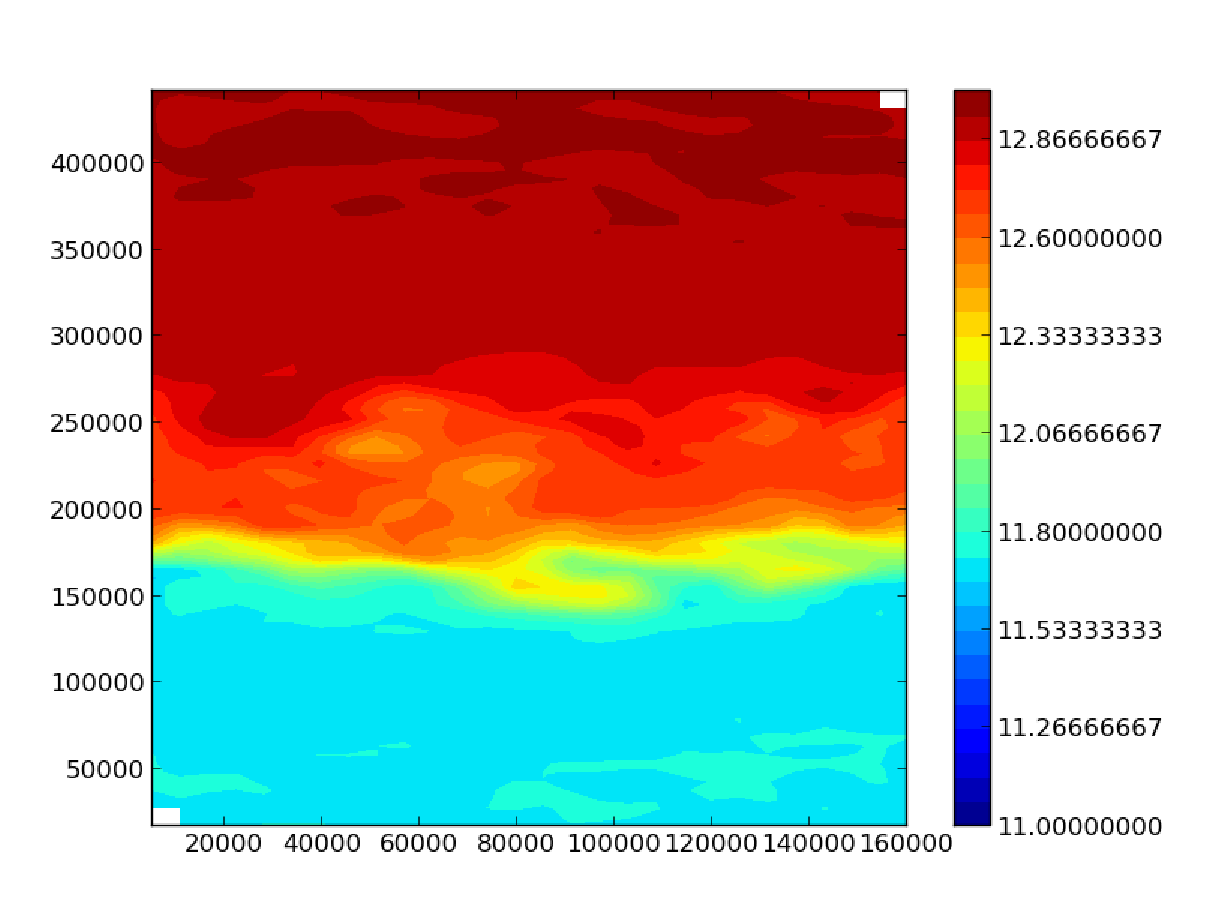
\includegraphics[scale=0.3]{ocean/figures/baroclinic_channel_10000m_20levs_10days.pdf}}
	\hfill
	\subfloat[4km horizontal resolution temperature field after 10 simulation days.]{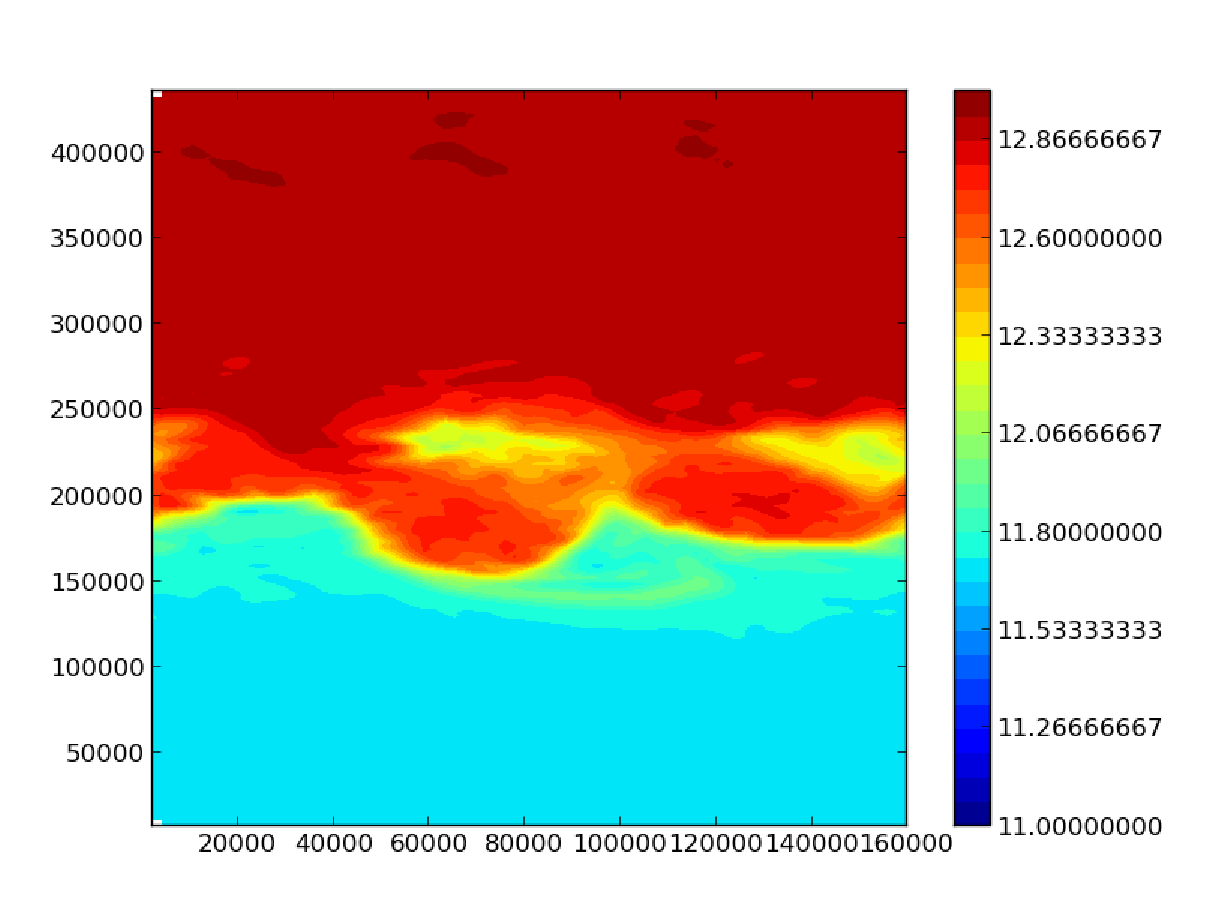
\includegraphics[scale=0.3]{ocean/figures/baroclinic_channel_4000m_20levs_10days.pdf}}
	\hfill
	\subfloat[1km horizontal resolution temperature field after 10 simulation days.]{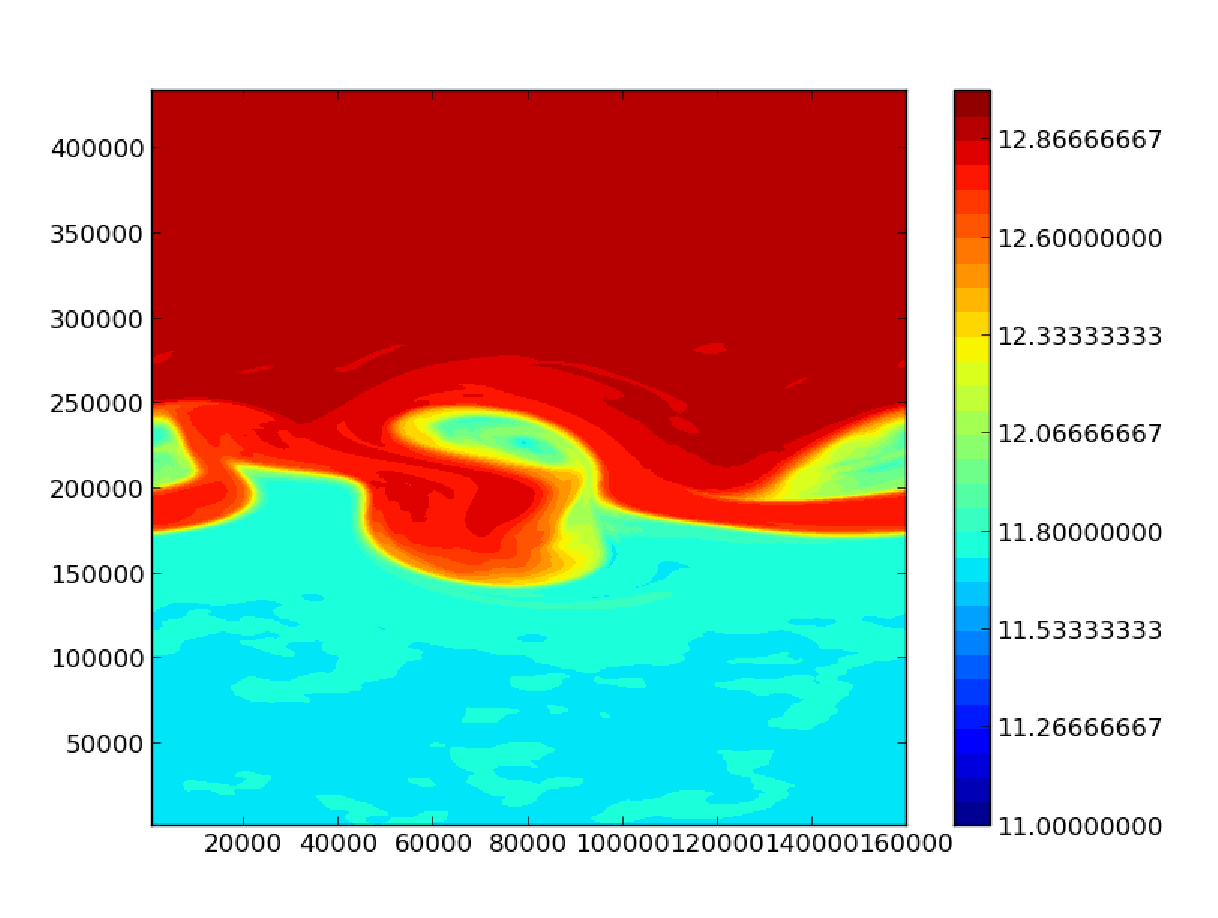
\includegraphics[scale=0.3]{ocean/figures/baroclinic_channel_1000m_20levs_10days.pdf}}
\end{figure}

